\documentclass[tikz, border=14pt]{standalone}
\usepackage{tikz}
\usepackage{mathtools}
\usetikzlibrary{bayesnet}
\begin{document}
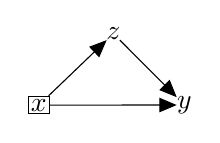
\begin{tikzpicture}
\tikzset{
    treat/.style = {
    draw = black,
        shape = rectangle,
        inner sep = 1pt
    }
    }
    \node[treat] (x) {$x$};
    \node[const, above right = of x] (z) {$z$};
    \node[const, below right = of z] (y) {$y$};
    \edge{x}{y};
    \edge{z}{y};
    \edge{x}{z};
\end{tikzpicture}
\end{document}